\documentclass[12pt,a4paper,titlepage]{article}
\usepackage[utf8]{inputenc}
\usepackage[spanish]{babel}
\usepackage[T1]{fontenc}
\usepackage[pdftex]{color,graphicx}
\usepackage{listings}
\usepackage{url}
\usepackage{titlesec}
\usepackage{tabularx}
\usepackage{hyperref}

\titleclass{\subsubsubsection}{straight}[\subsection]

\newcounter{subsubsubsection}
\renewcommand\thesubsubsubsection{\thesubsubsection.\arabic{subsubsubsection}}
\renewcommand\theparagraph{\thesubsubsubsection.\arabic{paragraph}} % optional; useful if paragraphs are to be numbered

\titleformat{\subsubsubsection}
  {\normalfont\normalsize\bfseries}{\thesubsubsubsection}{1em}{}
\titlespacing*{\subsubsubsection}
{0pt}{3.25ex plus 1ex minus .2ex}{1.5ex plus .2ex}

\makeatletter
\renewcommand\paragraph{\@startsection{paragraph}{5}{\z@}%
  {3.25ex \@plus1ex \@minus.2ex}%
  {-1em}%
  {\normalfont\normalsize\bfseries}}
\renewcommand\subparagraph{\@startsection{subparagraph}{6}{\parindent}%
  {3.25ex \@plus1ex \@minus .2ex}%
  {-1em}%
  {\normalfont\normalsize\bfseries}}
\def\toclevel@subsubsubsection{4}
\def\toclevel@paragraph{5}
\def\toclevel@paragraph{6}
\def\l@subsubsubsection{\@dottedtocline{4}{7em}{4em}}
\def\l@paragraph{\@dottedtocline{5}{10em}{5em}}
\def\l@subparagraph{\@dottedtocline{6}{14em}{6em}}
\makeatother

\setcounter{secnumdepth}{4}
\setcounter{tocdepth}{4}

\definecolor{gray}{RGB}{127,127,127}
\newcommand{\HRule}{\rule{\linewidth}{0.5mm}}

% Espacio entre párrafos
\setlength{\parskip}{0.2\baselineskip}

\lstset{
basicstyle=\ttfamily,                   	% Code font
stepnumber=1,                           	% Step between two line-numbers
numbersep=5pt,                          	% How far are line-numbers from code
frame=topbottom,                             	% A frame around the code
tabsize=4,                              	% Default tab size
captionpos=b,                           	% Caption-position = bottom
breaklines=true,                        	% Automatic line breaking?
breakatwhitespace=false,                	% Automatic breaks only at whitespace?
showspaces=false,                       	% Dont make spaces visible
showtabs=false,                         	% Dont make tabls visible
linewidth=\textwidth,                   	% Defines the base line width
}

\author{
	Daniel Garabato Míguez
	\and Vanesa López Beade
	\and Daniel Valcarce Silva
}
\title{Memoria Práctica LN}
\date{Curso 2012-2013}

\begin{document}

% Título
\begin{titlepage}
\begin{center}

\includegraphics[width=10cm]{res/logo_udc}\\
\vspace{1cm}
\textsc{\Large Lenguajes Naturales}\\[0.5cm]
\textsc{\Large Curso 2012/2013}\\[0.5cm]

\HRule \\[0.4cm]
{ \huge \bfseries My Little Trivial Player}\\[0.4cm]
{ \Large \bfseries Memoria de la Práctica}\\[0cm]

\HRule \\[0cm]
\end{center}

\vfill
\emph{Autores:}
\vspace{0.5cm}
\\
\vspace{0.1cm}
Garabato Míguez, Daniel \texttt{<daniel.garabato@udc.es>}\\
\vspace{0.1cm}
López Beade, Vanesa \texttt{<vanesa.lopezb@udc.es>}\\
\vspace{0.1cm}
Valcarce Silva, Daniel \texttt{<daniel.valcarce@udc.es>} (Portavoz)\\

\end{titlepage}


% Índice
\tableofcontents
\clearpage

%Cuerpo
\section{Introducción}
El objetivo de la presente práctica es realizar la implementación de un sistema de búsqueda de respuestas (\emph{question answering}). Para ello, en primer lugar, diseñaremos una arquitectura general del sistema en la que se especificará el objetivo de cada uno de los módulos.

Para implementar las distintas unidades funcionales de la práctica, implementaremos nuestros propios algoritmos, pero también haremos uso de múltiples herramientas de terceros. Describiremos dichas herramientas y para qué las hemos utilizado.

Consideraremos diferentes estrategias a la hora de resolver las diferentes problemáticas. Implementaremos aquellas que estén a nuestro alcance y las evaluaremos para quedarnos con las que nos den mejores resultados.

Se incluye en esta memoria un manual de instalación de la aplicación puesto que al hacer uso de múltiples herramientas de diferentes tecnologías es necesario la instalación de numerosos paquetes. Por otro lado, la memoria también contiene unas instrucciones de uso de la práctica.

\clearpage
\section{Arquitectura del sistema}
Basándonos en varios modelos conceptuales de un sistema de búsqueda de respuestas \cite{modelo1}, \cite{modelo2} y el dado en la asignatura, hemos desarrollado nuestra propia arquitectura que puede verse en la Figura \ref{fig:arquitectura}.

\begin{figure}[h!]
\begin{center}
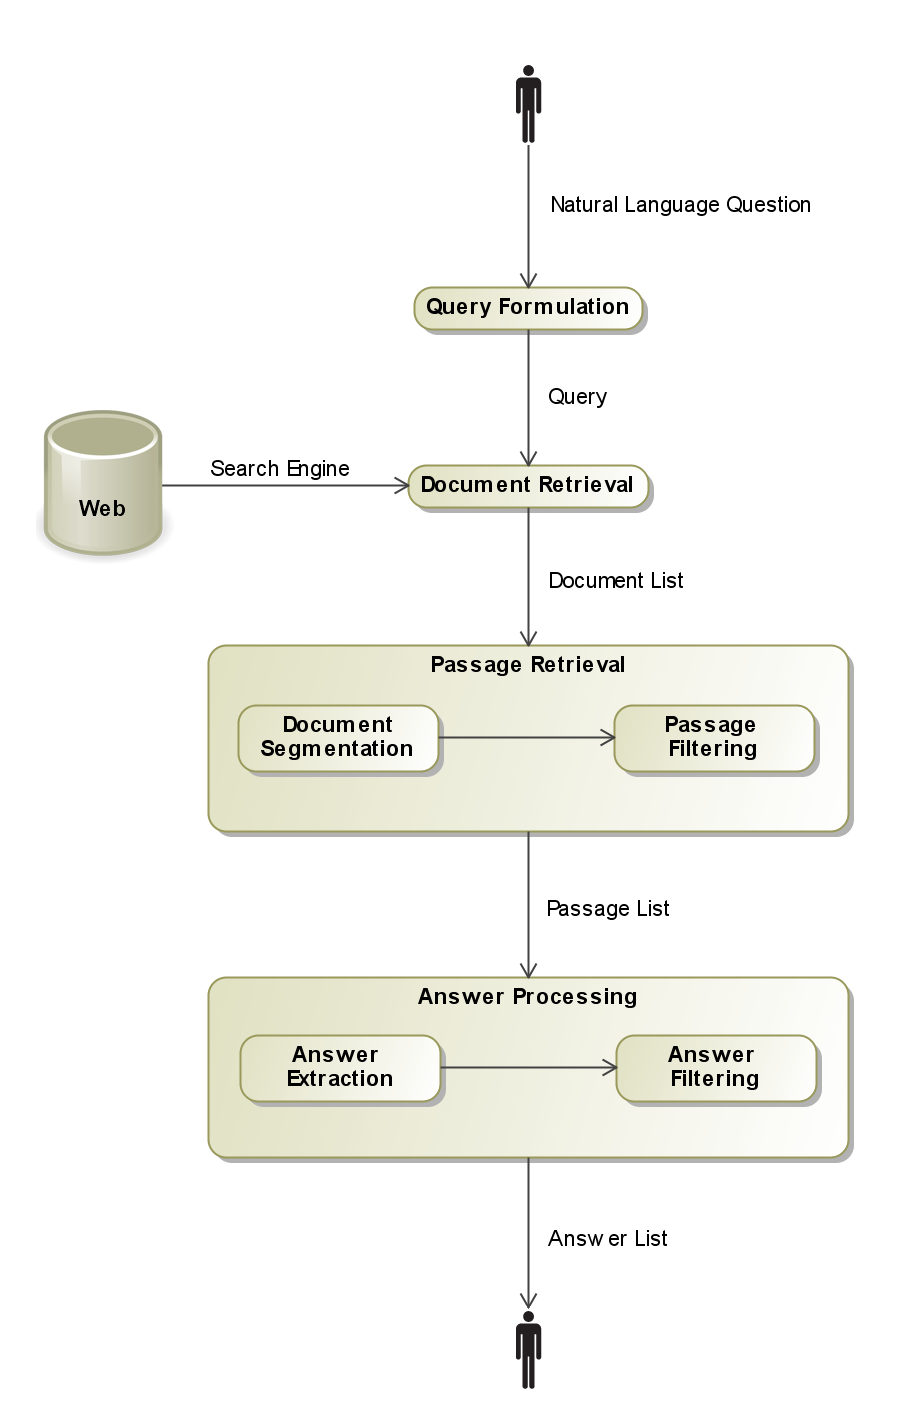
\includegraphics[width=0.9\textwidth]{res/arquitectura}
\end{center}
\caption{Arquitectura general del sistema}
\label{fig:arquitectura}
\end{figure}

\begin{description}
	\item[Query Formulation] A partir de una pregunta en lenguaje natural genera una consulta (\emph{query}) que será posteriormente interpretada por un motor de búsqueda web.
	\item[Document Retrieval] Obtiene una lista de documentos tras realizar la consulta pertinente en los motores de búsqueda.
	\item[Passage Retrieval] Devuelve los pasajes relevantes de la lista de documentos anterior.
		\begin{description}
			\item[Document Segmentation] Divide cada documento en pasajes.
			\item[Passage Filtering] Selecciona los pasajes más relevantes.
		\end{description}
	\item[Answer Procesing] Genera las respuestas asociadas a los pasajes relevantes.
		\begin{description}
			\item[Answer Extraction] Extrae las respuestas asociadas a cada pasaje.
			\item[Answer Filtering]	Filtra las mejores respuestas.
		\end{description}
\end{description}

\subsection{Vista estática}
En la Figura \ref{fig:clases} se muestra un diagrama de clases de nuestro sistema.

% % % % % % % % % %
% TODO: Completar %
% % % % % % % % % %

\begin{figure}[h!]
\begin{center}
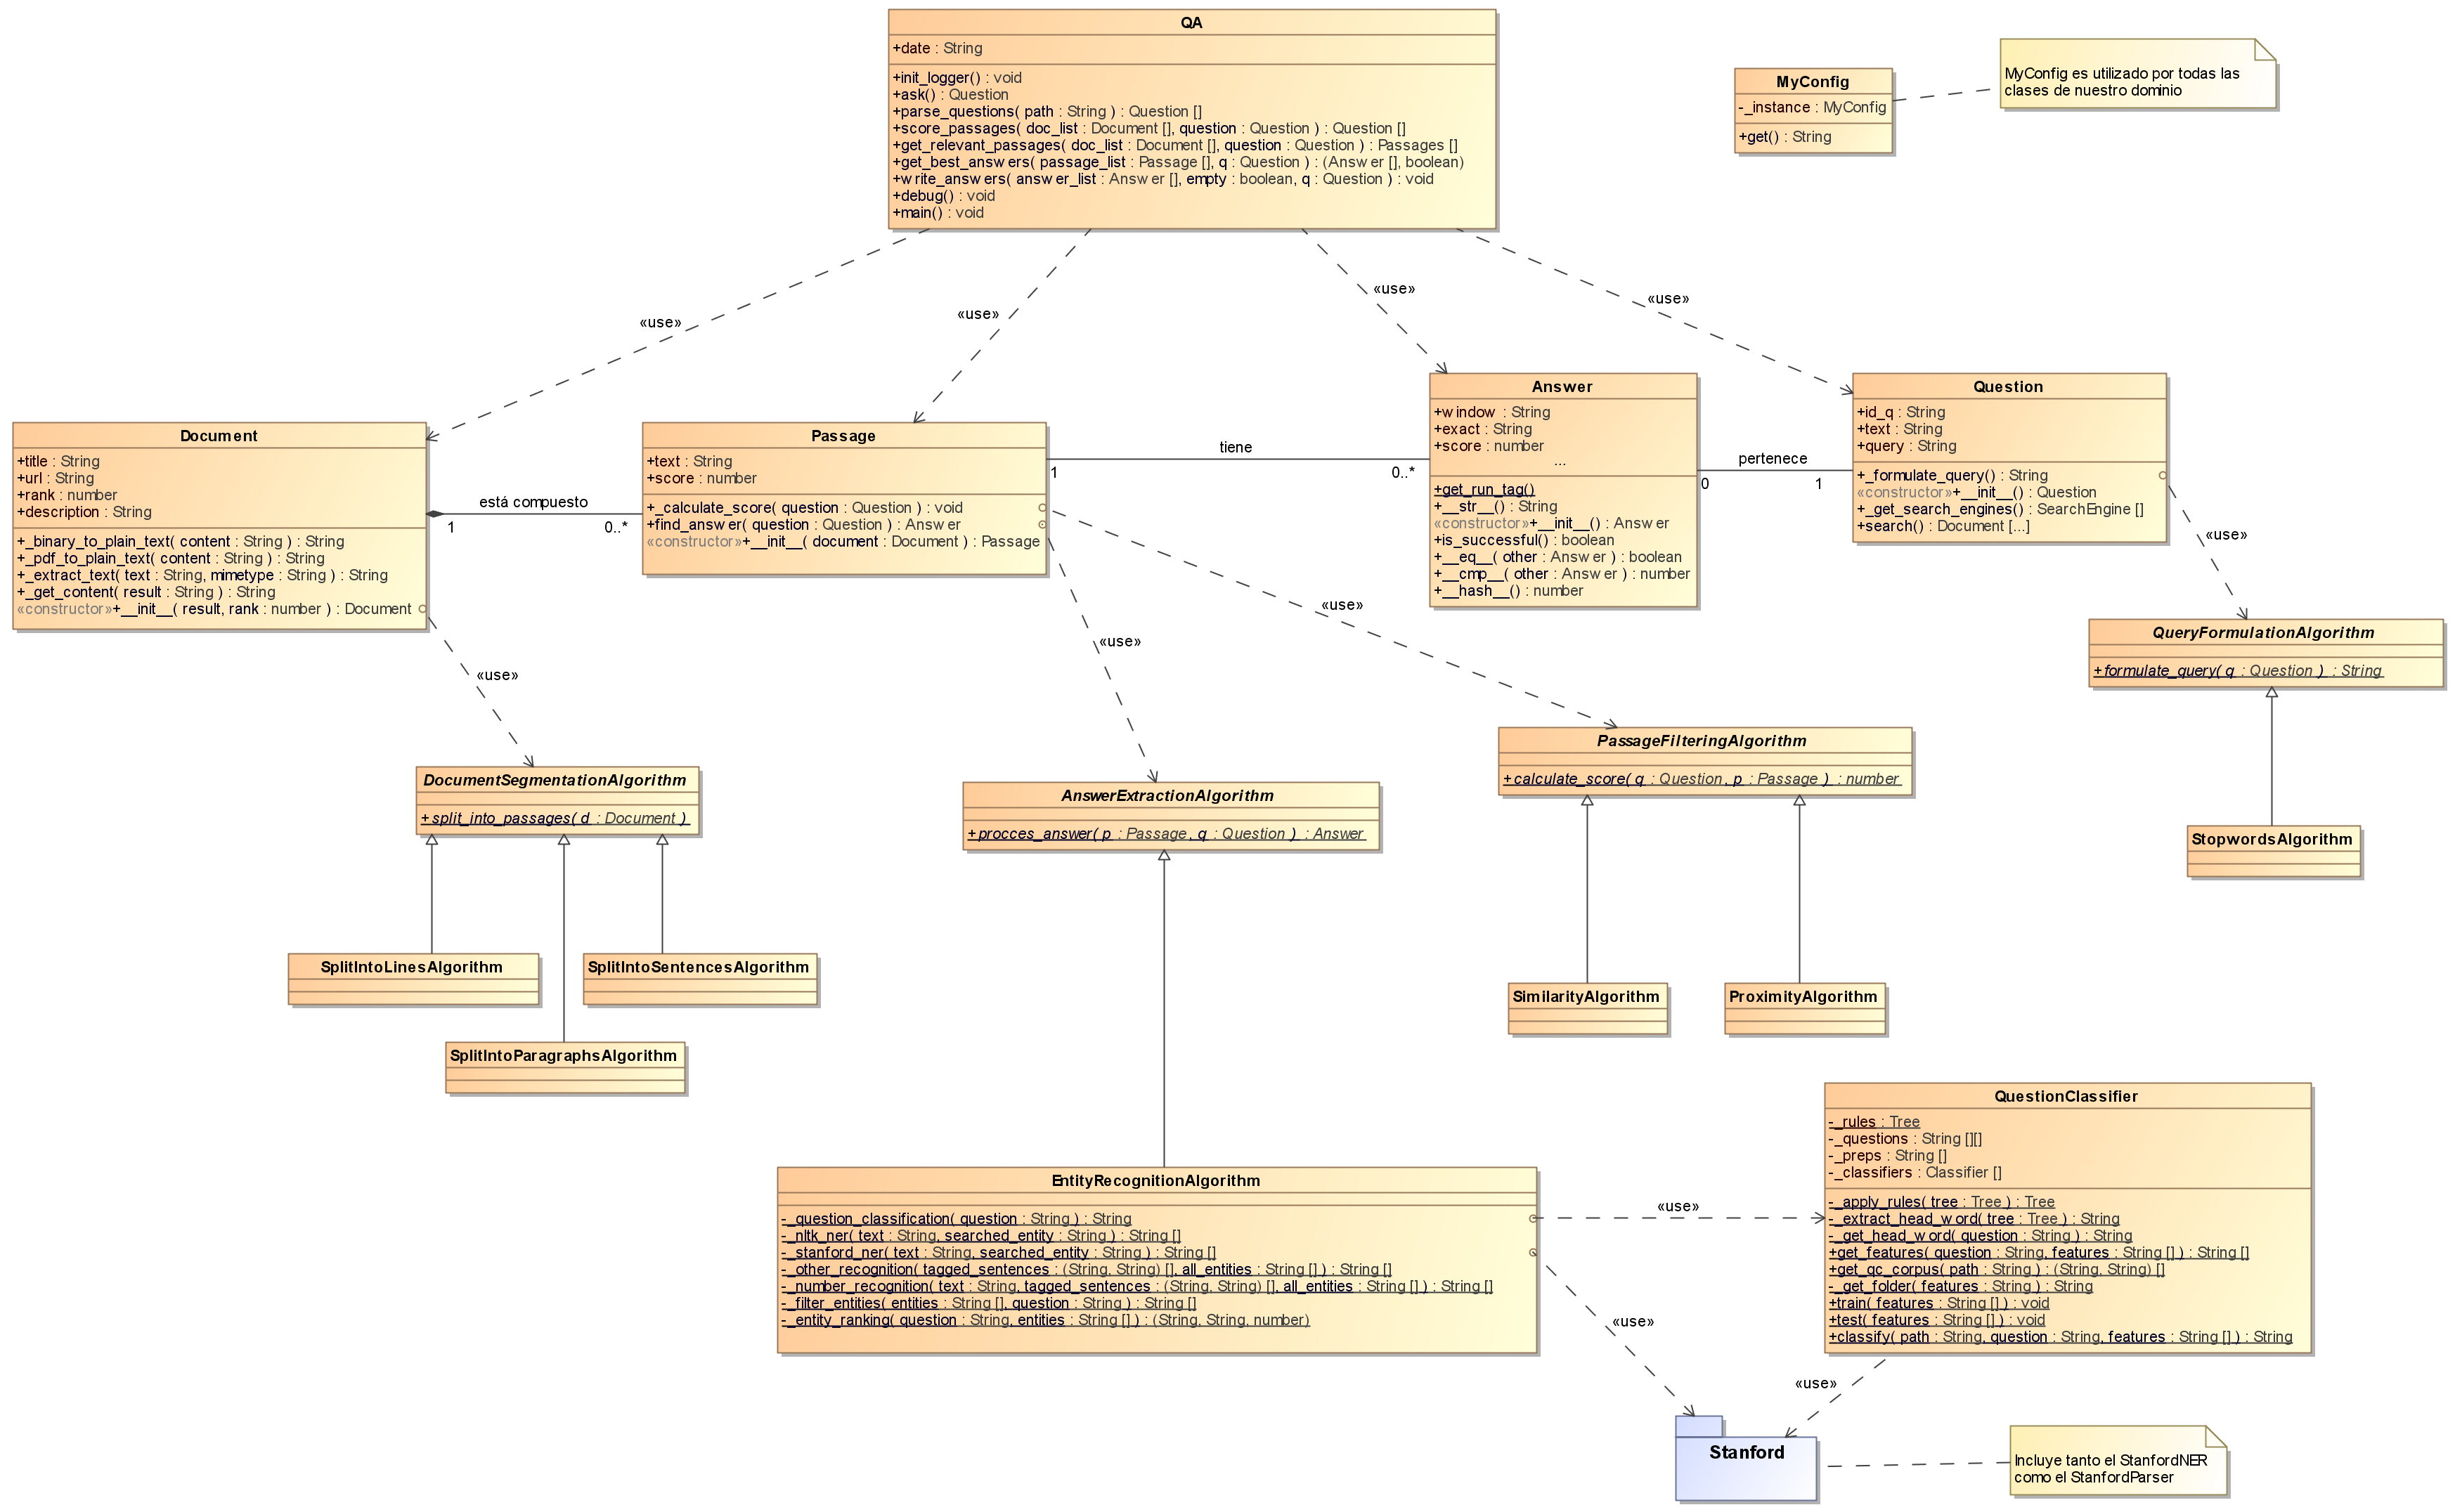
\includegraphics[angle=90,width=0.85\textwidth]{res/clases}
\end{center}
\caption{Diagrama de clases de la práctica}
\label{fig:clases}
\end{figure}

\subsection{Vista dinámica}
Para ilustrar el proceso de búsqueda de respuestas del sistema, hemos elaborado un diagrama de secuencia que puede verse en la Figura \ref{fig:secuencia}. En dicho diagrama se puede observar el flujo del programa durante la búsqueda de respuestas ante una pregunta realizada por el usuario por línea de comandos.

\begin{figure}[h!]
\begin{center}
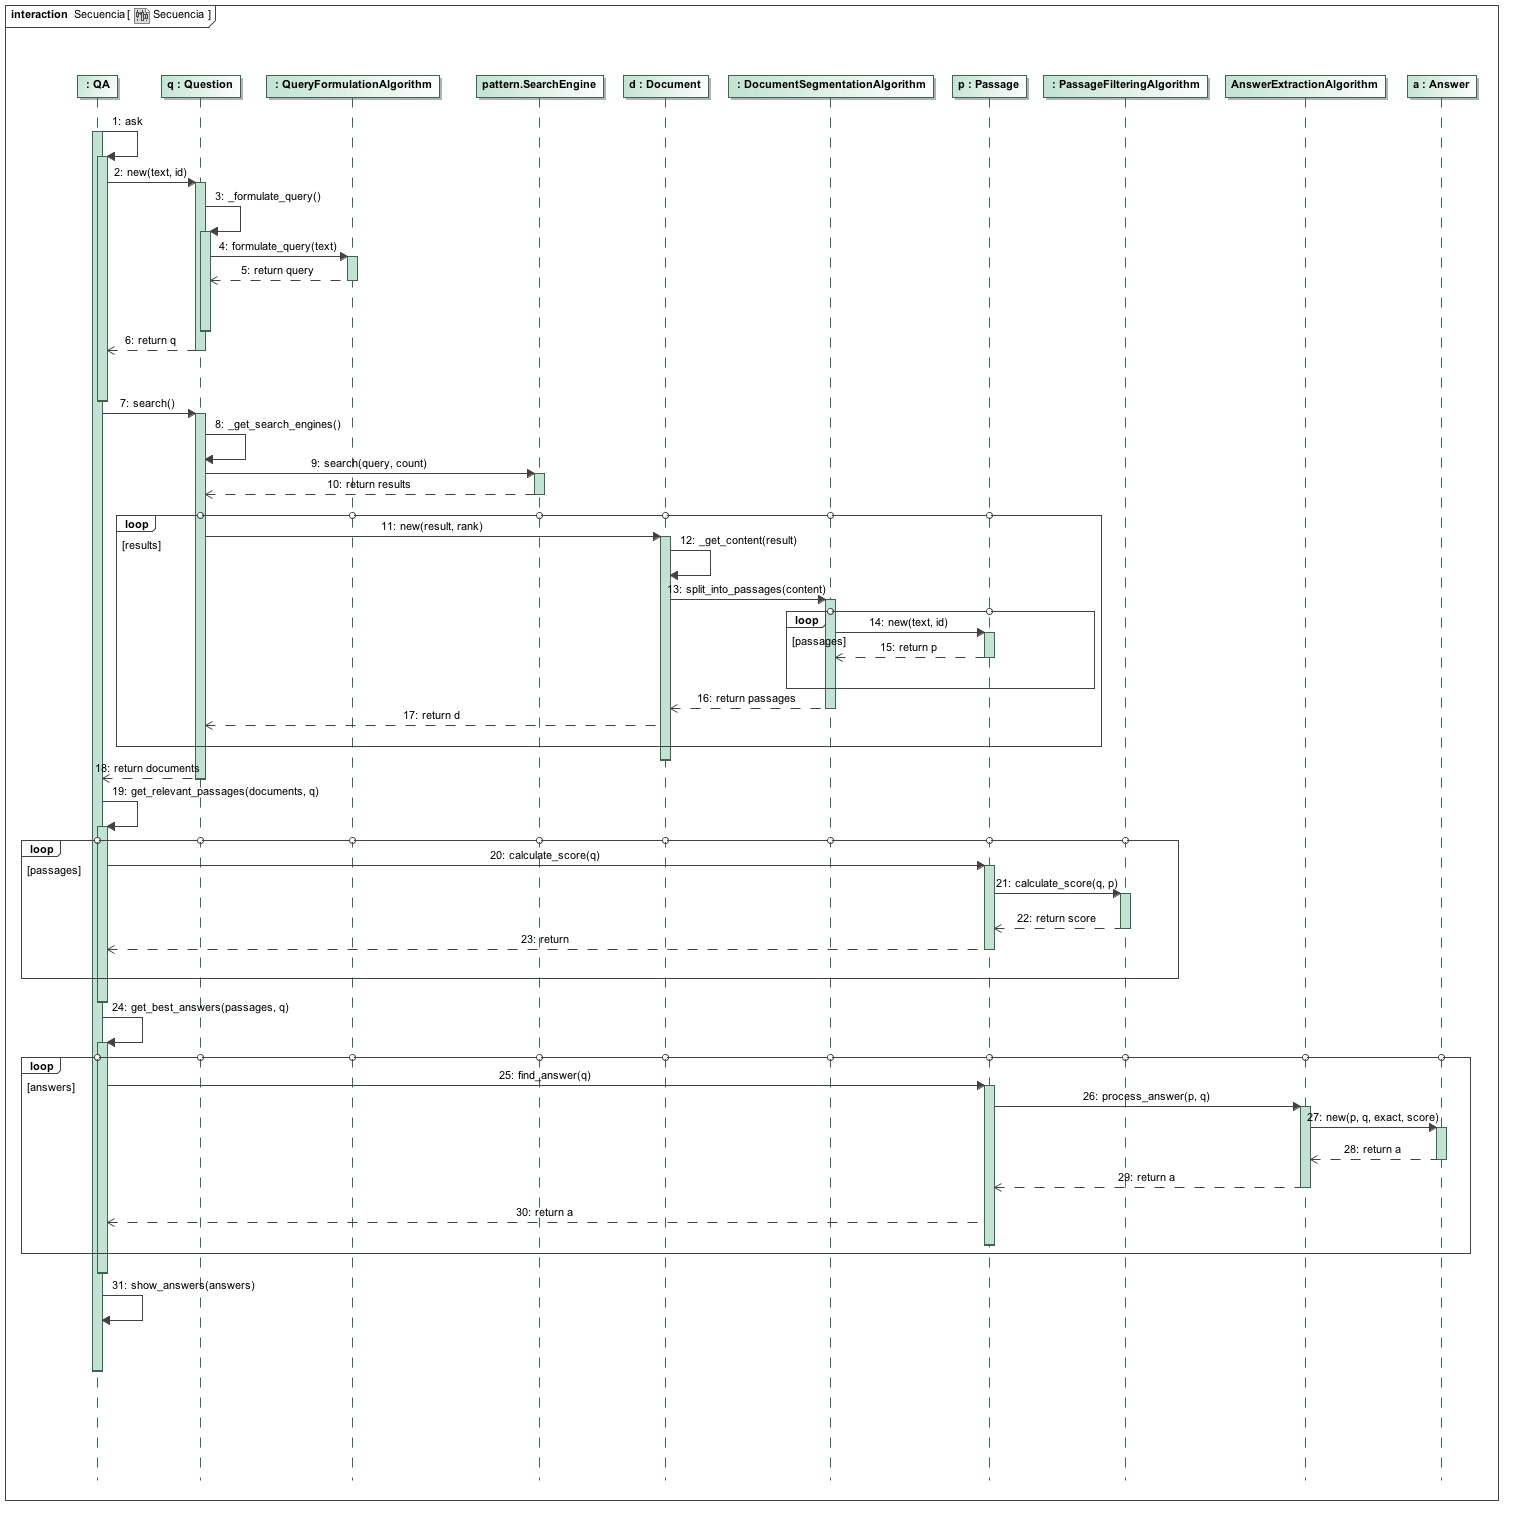
\includegraphics[width=\textwidth]{res/secuencia}
\end{center}
\caption{Diagrama de secuencia del proceso de búsqueda de respuestas}
\label{fig:secuencia}
\end{figure}

\clearpage
\section{Herramientas empleadas}
A continuación se muestran las herramientas utilizadas en el desarrollo de la práctica, bla, bla, bla...
% % % % % % % % % %
% TODO: Completar %
% % % % % % % % % %

\begin{description}
	\item[NLTK] Framework libre de procesamiento de lenguaje natural para Python. Puede descargarse en \cite{nltk}.
	\item[Pattern] Módulo de \emph{web mining} libre para Python. Puede descargarse en \cite{pattern}.
	\item[PDFMiner] Módulo de Python para la extracción de información de docuemntos PDF. Más información en \cite{pdfminer}.
	\item[lxml] Módulo de Python...
	\item[Stanford NER]
	\item[Stanford Parser]
	\item[Git] Sistema de control de versiones distribuido libre. Puede descargarse en \cite{git}.
	\item[BitBucket] Repositorio online para git. Puede accederse a él en \cite{bitbucket}.
	\item[\LaTeX] Sistema de composición de textos con el que se ha elborado el presente documento. Más información en \cite{latex}.

\end{description}


\clearpage
\section{Manual de instalación y uso}
En esta sección se describen los pasos a seguir para instalar correctamente todos los componentes necesarios para ejecutar nuestra práctica. Asimismo, también se adjuntan las intrucciones detalladas de uso.

A pesar de que las tecnologías utilizadas son multiplataforma, se recomienda utilizar un sistema operativo UNIX. Concretamente, se ha comprobado el correcto funcionamiento de la práctica en ArchLinux 2012.10.06, Debian 7.0, Mac OS X 10.8 y Ubuntu 11.04.

\subsection{Instalación del sistema}
A continuación se detallan los paquetes necesarios y cómo instalarlos.

\subsubsection{Python y sus módulos}
Es necesario disponer de una versión moderna de Python 2 (al menos Python 2.6, pero se recomienda Python 2.7). En el sitio web de Python se puede descargar el intérprete \cite{python}. Hemos utilizado únicamente el intérprete recomendado (CPython) con lo que no podemos garantizar el correcto funcionamiento en otras implementaciones como PyPy.

Una vez obtenido Python, es necesario instalar diversos módulos. Para simplificar el proceso, es preciso disponer de las SetupTools de Python. Hay scripts disponibles para diversas plataformas que pueden descargarse de su sitio web \cite{setuptools}.

\begin{lstlisting}
# sh path/to/downloads/setuptools-{version}.egg
\end{lstlisting}

Es preciso instalar Pip para instalar el resto de módulos:

\begin{lstlisting}
# easy_install pip
\end{lstlisting}

A continuación, instalamos los módulos Numpy, PyYAML, NLTK, PDFMiner, lxml y Pattern con Pip:

\begin{lstlisting}
# pip install -U numpy pyyaml nltk pdfminer lxml pattern
\end{lstlisting}

Es necesario bajarse los corpus del NLTK para que funcionen correctamente algunas de sus características como el PoS Tagger o el Named Entity Recognition Tagger:

\begin{lstlisting}
$ python
>>> import nltk
>>> nltk.download('all')
\end{lstlisting}


\subsubsection{Java}
Aunque nuestra práctica está realizada en Python, utilizamos herramientas del grupo Stanford NLP que están desarrolladas en Java. Estas requieren Java 6 o superior. En la web de Oracle se puede descargar el JDK \cite{java}.

Los componentes de Stanford que se son necesarios ya vienen incluidos con el código de la práctica por lo que no es necesario descargarse nada más.

\subsubsection{Claves de buscadores}
El módulo de obtención de documentos de la web requiere unas \emph{API Keys} de los buscadores a utilizar. En el fichero de configuración de la práctica ya se incluye por defecto unas claves gratuitas de Google y Bing que pueden ser sustituidas por otras claves válidas sin dificultad.

La clave de Google permite realizar 100 consultas por hora, mientras que la de Bing da acceso a 5000 consultas al mes.


\subsection{Uso del sistema}
El sistema tiene dos modos de funcionamiento principales así como un tercero con objetivos de \emph{debugging}. Con el objetivo de facilitar el uso de nuestro programa, se ha codificado un script en Bash (\texttt{launch.sh}) localizado en la raíz del proyecto que permite lanzar fácilmente la práctica.

En cualquiera de los tres modos de ejecución, las respuestas se almacenan en un fichero en la carpeta \texttt{res}. El nombre de dicho fichero se obtiene a partir del \emph{timestamp} de la hora de ejecución del programa.

\subsubsection{Modo interactivo}
El modo interactivo permite al usuario introducir una pregunta por la entrada estándar. El sistema buscará procesará la pregunta y devolverá la respuesta en el fichero de respuestas.

Para iniciar este modo, debemos ejecutar el script con la opción \emph{interactive}:
\begin{lstlisting}
$ ./launch.sh interactive
\end{lstlisting}

O bien ejecutar directamente el código Python:
\begin{lstlisting}
$ cd src
$ python QA.py
\end{lstlisting}

\subsubsection{Modo \emph{batch}}
Para el procesamiento de preguntas por lotes, nuestra práctica permite especificar un fichero en el que se leerán una serie de preguntas que serán procesadas secuencialmente. Los resultados de cada pregunta se encuentran todos en el mismo fichero.

El formato del fichero de preguntas es el siguiente. Cada pregunta se encontrarán en una línea y estará precedida por un código alfanumérico (sin blancos). A continuación de dicho código, el resto de la línea será considerado el cuerpo de la pregunta.

Este modo de ejecución puede ser invocado desde el script con la opción \emph{batch} seguido de la ruta del fichero de preguntas:
\emph{interactive}:
\begin{lstlisting}
$ ./launch.sh batch <file>
\end{lstlisting}

También se puede ejecutar directamente el código Python:
\begin{lstlisting}
$ cd src
$ python QA.py <file>
\end{lstlisting}

\subsubsection{Modo \emph{debug}}
Por último, nuestra práctica permite ejecutar el proceso de búsqueda de respuestas a partir de un conjunto de documentos ya obtenidos de los motores de búsqueda. El objetivo de esta modalidad de ejecución es limitar el número de consultas web durante la fase de pruebas debido a los límites de las claves gratuitas de Bing y Google.

Para que funcione correctamente este módulo, es necesario realizar en primer lugar una pregunta de modo interactivo o \emph{batch} con la opción \emph{persistence.document} activada en el fichero de configuracion (más información sobre cómo modificar la configuración de la práctica en la Sección \ref{section:conf}). Esto nos generará un fichero llamado \texttt{documentos.pkl} que contiene los documentos obtenidos serializados mediante el módulo Pickle de Python y que es necesario para la ejecución en modo \emph{debug}.

A continuación, solo se necesita ejecutar el script la opción \emph{debug}:
\begin{lstlisting}
$ ./launch.sh debug
\end{lstlisting}

Alternativamente, se puede ejecutar directamente el código Python:
\begin{lstlisting}
$ cd src
$ python QA.py pickle
\end{lstlisting}

\subsection{Fichero de configuración}
\label{section:conf}
Para dotar de mayor flexibilidad a la práctica, se han creado dos ficheros de configuración que permiten modificar el comportamiento de los diversos módulos y del sistema de \emph{logging}.

\subsubsection{\texttt{src/conf/config.conf}}
Permite modificar los parámetros de los diversos módulos del sistema de búsqueda de repuestas. Las posibles opciones se encuentran en forma de comentario dentro del fichero de configuración y tienen nombres autodescriptivos.

\subsubsection{\texttt{src/conf/logging.conf}}
El fichero de configuración del módulo Logging de Python permite establecer qué tipo de \emph{logs} se registran en ficheros de texto o por salida estándar. Para más información, consultar la referencia oficial del módulo \cite{logging}.

\clearpage
\section{Algoritmos}
En esta sección se detallan los algoritmos utilizados en el sistema de búsqueda de respuestas.
% % % % % % % % % %
% TODO: Completar %
% % % % % % % % % %

\subsection{Query Formulation}
El objetivo de estos algoritmos es formular una consulta para los buscadores web a partir de la pregunta introducida por el usuario.

\subsubsection{Stopwords}
Este algoritmo nos devuelve una query. Es llamado cada vez que se crea un objeto de tipo Question y recibe el texto de la pregunta. Su funcionamiento consiste en primero pasar el texto de la pregunta a minúsculas y , a continuación, obtenemos una lista con los caracteres de la pregunta. De esta lista eliminamos los símbolos que no nos interesan (comas, interrogaciones, exclamaciones, etc.) puesto que no nos influyen en la búsqueda. Tenemos así el texto de la pregunta filtrado.

Finalmente obtenemos otra lista con las palabras de la pregunta y, utilizando el corpus del NLTK con las \emph{stopwords}, eliminamos las palabras irrelevantes a la hora de realizar la búsqueda. Tenemos así nuestra query lista para pasársela a los buscadores.

\subsection{Document Segmentation}
Los siguientes algoritmos son llamados cada vez que se crea un objeto de tipo Documento; les pasaremos un documento y nos devolverán la lista de pasajes de dicho documento.

\subsubsection{Split into Lines}
En este primer algoritmo obtenemos pasajes compuestos por un número fijo de líneas ( a determinar por el usuario, en caso de fallo al obtenerlo, dicho número será 5 ) del documento superponiendo dichos pasajes. Para ello, se divide el contenido del documento en líneas y se itera sobre estas líneas de manera que cada pasaje estará formado por el número de líneas fijado. En cada nueva iteración, un pasaje estará formado por dicho número de líneas menos una del pasaje de la iteración anterior más una nueva línea. Por último se añade también como pasaje la descripción que nos ofrece el motor de búsqueda ya que puede resultar relevante según la lógica del buscador.

\subsubsection{Split into Paragraphs}
En este segundo caso, la forma de obtener pasajes cambia para obtener en cada pasaje un único párrafo. Se divide el contenido del documento en líneas y cada pasaje estará formado por una de ellas. Añadiendo además, como en el caso anterior, el pasaje formado por la descripción ofrecida por el motor de búsqueda.

\subsubsection{Split into Sentences}
Por último, este algoritmo obtiene pasajes formados por el número de frases indicadas por el usuario. El contenido del documento se divide en frases utilizando el sent\_tokenize del NLTK. Se añade además, como en los dos casos anteriores, el pasaje formado por la descripción ofrecida por el motor de búsqueda.

\subsection{Passage Filtering}
Estos algoritmos fijarán una determinada puntuación a cada pasaje según su relevancia para una determinada pregunta para así poder seleccionar los mejores.

\subsubsection{Similarity}
En primer lugar, al texto de la pregunta y del pasaje les eliminamos las stopwords con el algoritmo de Query Formulation: Stopwords y dividimos ambos textos en palabras, obteniendo dos listas. A continuación, aplicamos stemming sobre ambas listas, obtenemos las palabras que están en ambas listas y este número de palabras coincidentes será nuestra puntuación inicial.

Por último, los pasajes que pertenezcan a documentos obtenidos de respuestas situadas en las posiciones más altas del ranking de respuestas devueltas por los motores de búsqueda obtendrán mayor puntuación por considerarse que esto indica que son mejores. Normalizamos el ranking del documento al que pertenece el pasaje que estamos puntuando y multiplicamos la puntuación inicial anterior por esta cantidad, obteniendo así, la puntuación final del pasaje.

\subsubsection{Proximity}
Como en el caso del algoritmo anterior primero eliminamos las stopwords con el algoritmo de Query Formulation: Stopwords, dividimos ambos textos en palabras y aplicamos stemming tanto sobre la lista de palabras de la pregunta como la de palabras del pasaje.

A la hora de puntuar los pasajes se valora que estos tengan palabras de la pregunta cercanas entre si, asignándole una puntuación de acuerdo a lo próximas que estén entre sí.

\subsubsection{Mixed}
Consideramos en este algoritmo una estrategia mixta, asignándole a cada pasaje la media de la puntuación obtenida con los dos algoritmos anteriores (Similarity y Proximity).

\subsection{Answer Extraction}
Los algoritmos de extracción de respuestas tienen como objetivo hallar una respuesta dados una pregunta y un pasaje relevante.

\subsubsection{Entity Recognition}
\label{s:ne_recog}
El funcionamiento de este algoritmo se basa en la extracción de entidades del texto de un pasaje. Para ello, en primer lugar, obtenemos la clasificación de la pregunta y, a continuación, recuperamos las entidades adecuadas a dicha clasificación.

Para cada pasaje, devolvemos la entidad que más se repite en la pregunta con una puntuación que determina su frecuencia de aparición en el pasaje.

\subsubsubsection{Question Classification}
Realizamos una clasificación de la pregunta para saber qué tipo de entidades debemos obtener del pasaje. Para ello hemos entrenado diferentes clasificadores a partir de un corpus de entrenamiento formado por preguntas y su clasificación en Other, Number, Person, Location, Time, Date, Money, Percent y Organization.

Hemos utilizado tres tipos de clasificadores: de Bayes ingenuo, de árbol de decisión y de máxima entropía. A su vez, hemos utilizado diferente combinaciones de las siguientes características: primera palabra, primer sustantivo y \emph{head word}.

Para obtener la \emph{head word}, es decir, la palabra clave que indica el tipo de pregunta hemos utilizado el algoritmo descrito en \cite{tesis:qc} y \cite{paper:qc}.

Tras probar todas las combinaciones posibles de clasificadores y características, el que mejor resultados da en el conjunto de test ha sido el clasificador bayesiano ingenuo con todas las características.

\subsubsubsection{Named Entity Recognition}
Una vez obtenida la clasificación de la pregunta, debemos buscar las entidades de ese tipo. Para ello, utilizamos el NER Parser de Stanford que permite la extracción de entidades tipo Time, Location, Organization, Person, Money, Percent y Date; sin embargo, debemos definir estrategias diferentes para los Number y los Other.

Para reconocer entidades Number utizamos el Part-of-Speech Tagger del NLTK obteniendo los numerales cardinales y ordinales (CD y JJ) y una expresión regular que reconoce caracteres numéricos.

Por último, la extracción de entidades tipo Other se realiza obteniendo los sustantivos comunes que no son entidades tras un análisis léxico por parte del NLTK.

Descartamos aquellas respuestas que son palabras que ya aparecen en la pregunta.

También es posible emplear el extractor de entidades del NLTK (se puede indicar en el fichero de configuración); no obstante, hemos visto que proporciona peores resultados.

\clearpage
\section{Resultados}
En las siguientes tablas se muestran los resultados obtenidos para las pruebas realizadas. Nos quedamos con la cuarta configuración puesto que es con la que obtenemos un mayor MRR.

\begin{table}[h!]
\begin{center}
\begin{tabular}{|c|c|c|c|}
\hline
Id & Document Retrieval & Document Segmentation & Passage Filtering\\\hline
1 & 10 resultados & sentences/5/100 & mixed\\\hline
2 & 10 resultados & paragraph/-/100 & mixed\\\hline
3 & 10 resultados & sentences/1/200 & mixed\\\hline
4 & 20 resultados & sentences/1/500 & mixed\\\hline
5 & 20 resultados & sentences/1/500 & proximity\\\hline
6 & 20 resultados & sentences/1/500 & similarity\\\hline
7 & 20 resultados & sentences/5/100 & mixed\\\hline
8 & 20 resultados & sentences/5/100 & proximity\\\hline
9 & 20 resultados & sentences/5/100 & similarity\\\hline
\end{tabular}
\end{center}
\end{table}

\begin{table}[h!]
\begin{center}
\begin{tabular}{|c|c|c|c|c|}
\hline
Id & run-tag & MRR estricto & MRR permisivo & Respuestas R\\ \hline
1 & plnaex031ms & 0,24333 & 0,24333 & 15\\ \hline
2 & plnaex031ms & 0,19667 & 0,19667 & 11\\ \hline
3 & plnaex031ms & 0,31 & 0,31 & 19\\ \hline
4 & plnaex031ms & 0,32333 & 0,32333 & 18\\ \hline
5 & plnaex031ms & 0,26 & 0,26 & 16\\ \hline
6 & plnaex031ms & 0,29 & 0,29 & 17\\ \hline
7 & plnaex031ms & 0,28 & 0,28 & 16\\ \hline
8 & plnaex031ms & 0,19 & 0,21 & 11 \\ \hline
9 & plnaex031ms & 0,22667 & 0,22667 & 13\\ \hline
\end{tabular}
\end{center}
\end{table}

\begin{table}[h!]
\begin{center}
\begin{tabular}{|c|c|c|c|c|c|}
\hline
Id & R o U & NILs & NILs correctos & \% R & \% R o U\\ \hline
1 & 15 & 1 & 0 & 30,00\% & 30,00\% \\ \hline
2 & 11 & 1 & 0 & 22,00\% & 22,00\% \\ \hline
3 & 19 & 1 & 0 & 38,00\% & 38,00\% \\ \hline
4 & 18 & 1 & 0 & 36,00\% & 36,00\% \\ \hline
5 & 16 & 1 & 0 & 32,00\% & 32,00\% \\ \hline
6 & 17 & 1 & 0 & 34,00\% & 34,00\% \\ \hline
7 & 16 & 1 & 0 & 32,00\% & 32,00\% \\ \hline
8 & 12 & 1 & 0 & 22,00\% & 24,00\% \\ \hline
9 & 13 & 2 & 0 & 26,00\% & 26,00\% \\ \hline
\end{tabular}
\end{center}
\end{table}






\clearpage
\section{Diario de trabajo}
A continuación se muestra un resumen del trabajo realizado a lo largo de la elaboración de la presente práctica. Las entradas se ordenan por su fecha cronológica y describen brevemente las decisiones y las acciones tomadas.


\subsection{Jornada del 2012/10/26}
En la primera reunión del grupo, hemos discutido sobre los primeros pasos a la hora de enfrentar la práctica. Tras un análisis de los diferentes \emph{toolkits} que se nos presentan en el enunciado de la práctica, nos decidimos a usar NLTK por dos razones principales. El primer motivo es la gran cantidad de módulos que posee y su amplia documentación. En segundo lugar, porque Python nos parece un lenguaje muy cómodo para el desarrollo del proyecto.

Profundizando más en el desarrollo del trabajo, decidimos usar Git como sistema de control de versiones y apoyarnos en un repositorio privado de Bitbucket. Esto nos permitirá tener nuestro código bien organizado y documentado así como proporcionarnos un respaldo de los datos.

Por último, acordamos documentarnos más sobre el uso de Python en el procesamiento de lenguaje natural en general y con NLTK en particular. Para ello recurriremos a la bibliografía recomendada por los creadores del toolkit \cite{nltk-book}. También optamos por estudiar las APIs de Google y de Bing para realizar consultas.

\subsection{Jornada del 2012/10/29}
Hemos instalado y configurado NLTK. Hemos estudiado utilizar el módulo Pattern (en Python) para la implementación de las consultas en los buscadores (Google y Bing). Hemos solicitado unas claves para poder utilizar las APIs de dichos buscadores.

Por otro lado, hemos comenzado a estudiar la formulación de la consulta (\emph{query formulation}). Debemos eliminar aquellas palabras innecesarias (\emph{stopwords}) por lo que utilizamos el diccionario de Porter ya integrado en NLTK. Consideramos mantener las comillas y los apóstrofes ya que dan mejores resultados en los buscadores. Optamos por no eliminar la interrogación final puesto que es irrelevante para ellos.

\subsection{Jornada del 2012/11/05}
Se ha dedicado la tarde del presente día a la implementación de la búsqueda de información en los buscadores web (a saber, Google y Bing). Hemos comenzado empleando la biblioteca Pattern\cite{pattern} la cual nos aporta una interfaz adaptador entre el API de los buscadores y nuestro sistema. No obstante, tras las pruebas iniciales comprobamos que el servidor de Google devolvía un error HTTP400 Bad Request a nuestras peticiones.

Al no encontrar solución a este problema, dedujimos que sería un bug en la biblioteca Pattern por lo que comenzamos a desarrollar nuestra propia biblioteca para integrar las APIs de los buscadores. Tras la integración del API de Google, verificamos en las pruebas que se producía el mismo error. Buscando posibles soluciones en la web, averiguamos que el origen del error 400 no era una petición HTTP mal formada si no un error de autenticación: la clave del API que estábamos utilizando era incorrecta.

Comprobamos que efectivamente ese era el error y decidimos volver a utilizar la biblioteca Pattern en vez de seguir implementando la nuestra porque esta ya nos proporciona una acceso unificado a la información de los buscadores.

\subsection{Jornada del 2012/11/06}
Se ha realizado la planificación de la arquitectura del sistema de búsqueda de respuetas con el objetivo de orientar el desarrollo de los componentes que faltan. Hemos concluido crear las clases \texttt{QA}, \texttt{Query}, \texttt{Document}, \texttt{Passage} y \texttt{Answer} tras un esbozo del diagrama de clases que se ha construido a partir de un estudio de los casos de uso.

\subsection{Jornada del 2012/11/12}
Durante la sesión de hoy hemos continuado refinando nuestro sistema realizando una adaptación de las funcionalidades ya implementadas a la arquitectura del sistema esbozada en la sesión previa.

Además se ha implementado una sencilla interfaz para la realización de las consultas. Por un lado, se ofrece la posibilidad de introducir una única consulta manualmente en el sistema y, por otro lado, permitiremos el uso de un fichero externo para realizar múltiples consultas mediante el paso de un fichero como parámetro en nuestro programa principal. El tratamiento de dicho fichero de preguntas se realiza mediante una expresión regular con el fin de proporcionar mayor robustez al sistema.

En último lugar desarrollamos la lógica necesaria para gestionar un fichero de configuración.

\subsection{Jornada del 2012/11/13}
En primer lugar, hemos decidido crear una clase \texttt{MyConfig} cuyo objetivo es encapsular la forma de acceder al fichero de configuración.

A continuación hemos utilizado el módulo pickle de Python para serializar los documentos resultantes de realizar la consulta en los buscadores.

Por último, se ha desarrollado código capaz de manejar distintos tipos de documentos que nos podemos encontrar por la red:
\begin{itemize}
\item Los ficheros HTML se tratan con un procesador dedicado a ello que elimina las etiquetas, el código CSS o JavaScript, etc.
\item Los archivos en texto plano no necesitan procesamiento.
\item Aquellos documentos cuyo formato no reconocemos\footnote{En un inicio pensamos en tratar de forma especial documentos ofimáticos (.doc, .docx, .xls, .xlsx, .ppt, .pptx, OpenDocument...); sin embargo, la probabilidad de encontrárselos como resultado de la búsqueda generada por una pregunta factual es muy baja y el tratamiento genérico que hemos implementado da unos resultados satisfactorios.} son manejados de una forma genérica: mediante una expresión regular extraemos los caracteres legibles de los mismos.
\end{itemize}

\subsection{Jornada del 2012/11/19}
Hemos comenzado con la división de los documentos en pasajes. Consideramos oportuno que los fragmentos sean solapados para evitar la posible pérdida de información. En principio hemos decidido segmentar los documentos por líneas ---el número de ellas será especificado en el fichero de configuración---.

Posteriormente, se ha implementado el uso de logs mediante el módulo logging de Python. Hemos creado un fichero de configuración para tal efecto.

\subsection{Jornada del 2012/11/20}
En primer lugar, hemos reestructurado el proyecto para utilizar el patrón estrategia para los algoritmos de formulación de consultas, puntuación de pasajes y procesamiento de respuestas.

Hemos desarrollado nuestra primera heurística para la evaluación de la relevancia de los pasajes en la búsqueda de respuestas. El algoritmo se basa en la similitud entre el pasaje y la pregunta. Se limpia la pregunta y el pasaje de símbolos y stopwords. A continuación se calcula el número de palabras coincidentes. Dividimos dicha cantidad entre el número de palabras en el pasaje y lo ponderamos por la relevancia del resultado según el buscador.

Por otro lado, se ha refinado el algoritmo de formulación de consultas eliminando símbolos no deseados.

\subsection{Jornada del 2012/11/26}
Decidimos utilizar otro patrón estrategia para la segmentación del texto en pasajes. Creamos una estrategia nueva que segmenta el texto en párrafos, complementando asi a la estrategia de segmentar por un número fijo de líneas.

Mejoramos el algoritmo de filtrado de pasajes relevantes por similitud aplicando \emph{stemming} a la pregunta y al pasaje mediante el uso del Stemmer de Porter. Probamos además el uso de un lematizador basado en WordNet, pero tras su prueba descartamos su utilización ya que discriminaba menos casos similares.

Documentamos el fichero de configuración con los posibles algoritmos a emplear (formulación de consultas, segmentación en pasajes, búsqueda de pasajes relevantes y procesamiento de respuestas).

Implementamos lógica adicional para la gestión de las respuestas y su correcta visualización de acuerdo a las normas del enunciado de la práctica.

\subsection{Jornada del 2012/11/27}
Durante el día de hoy se ha diseñado el gráfico de arquitectura del sistema, estableciendo los diferentes módulos que componen el mismo:

\begin{itemize}
\item Query Formulation
\item Document Retrieval
\item Passage Retrieval
	\begin{itemize}
	\item Document Segmentation
	\item Passage Filtering
	\end{itemize}
\item Answer Processing
	\begin{itemize}
	\item Answer Extraction
	\item Answer Filtering
	\end{itemize}
\end{itemize}

Así mismo hemos elaborado un diagrama de secuencia en el que se expone el funcionamiento global del sistema (puesto que éste solo contempla un único caso de uso: realizar consultas).

\subsection{Jornada del 2012/12/03}
Corrección de múltiples errores en diferentes módulos de la práctica.

Hemos considerado que una consulta en diferentes motores de búsqueda nos puede dar los mismos documentos como resultado; por tanto, se ha decidido controlar la posible repetición de documentos para evitar duplicados.

\subsection{Jornada del 2012/12/04}
Añadimos la escritura de resultados en un fichero.

Implementamos la lógica necesaria para gestionar la posible falta de respuestas. Por un lado, si los motores de búsqueda no nos devuelven resultados deolvemos NIL con la puntuación máxima. Por otro lado, si no encontramos una buena respuesta en los documentos de la web devolvemos NIL con la puntuación mínima. Por último si el número de respuestas admisibles es menor que tres, las mostramos y añadimos un NIL con puntuación mínima.

En el fichero de configuración, podemos especificar el umbral de lo que consideramos una respuesta admisible.

\subsection{Jornada del 2012/12/10}
Creamos un algoritmo de Answer Extraction basado en la técnica de Named Entities Recognition explicado en la Sección \ref{s:ne_recog}. Queda por completar la parte de Query Classification (de momento solo admitimos preguntas sobre personas).

Mejoramos nuestra metodología de Answer Filtering ponderando las puntuaciones de las respuestas por su frecuencia relativa de aparición en los pasajes relevantes.

Realizamos las primeras pruebas sobre un sistema ya funcional y obtenemos buenos resultados ---en principio--- para preguntas relacionadas con personas. Las respuestas están motivadas correctamente y la tasa de aciertos ronda el 20\\%. Consideramos esto un hito en el desarrollo del sistema ya que tenemos una primera versión preliminar que proporciona resultados coherentes.

\subsection{Jornada del 2012/12/11}
Dedicamos el día de hoy a implementar técnicas de Question Classification. Utilizamos dos modelos: un clasificador bayesiano ingenuo y un modelo de máxima entropía proporcionados por NLTK.

Modificamos el corpus qc del NLTK para que se adapte a nuestras entidades y entrenamos ambos sistemas. Obtenemos una precisión algo más elevada en el caso del modelo de máxima entropía.

Consideramos realizar para el próximo día la integración del Named Entity Recognizer de Stanford puesto que los resultados del reconocedor de entidades del NLTK no son muy satisfactorios en algunos casos.

\subsection{Jornada del 2012/12/17}
Hemos implementado dos técnicas para detectar números y otros tipos de entidades (NUMBER y OTHER, respectivamente). Los números se reconocen como caracteres numérico o como sustantivos y adjetivos numerales. El reconocimiento de otro tipo de entidades se realiza mediante la extración de sustantivos (exceptuando aquellos que son entidades).

Realizamos también pequeñas refactorizaciones del código. Optimizamos la técnica de Question Classification mediante el uso de una caché de preguntas.

\subsection{Jornada del 2012/12/18}
En el día de hoy, se ha integrado el Named Entity Recognition de Stanford con el código actual mediante comunicación via un socket TCP. Ahora podemos utilizar ambos reconocedores de entidades (será necesario realizar una comparativa entre ellos).

\subsection{Jornada del 2012/12/26}
Concertamos una reunión con el profesor responsable de las prácticas para realizar un seguimiento de la misma y plantearle unas dudas sobre el reconocimiento de entidades tipo Other.

Realizamos correciones menores en el soporte de Unicode, el timeout de descarga de ficheros, el salvado de resultados en ficheros, la selección mediante el fichero de configuración del tipo de motor de NER o la falta de clasificadores de preguntas.

Por otro lado, hemos mejorado el Passage Retrieval consdirando también los snippets que nos proporcionan los buscadores como posibles pasajes relevantes. También modificamos la lógica del Answer Extraction para eliminar aquellos términos que ya aparecen en la pregunta como posibles respuestas (no nos van a preguntar de qué color es el caballo blanco de Santiago).

Tras realizar unas pruebas para evaluar la calidad de nuestro sistema, observamos que si el Question Classification falla, es imposible obtener una respuesta válida. Por tanto, nos hemos propuesto mejorarlo con la inclusión de más \emph{features} a nuestros clasificadores. Hemos probado con añadir un segundo sustantivo, pero vimos que empeoraba el rendimiento en el conjunto de test. A continuación, intentamos aproximarnos al problema utilizado chunking para obtener la \emph{head word} más característica; sin embargo, la calidad del análisis sintáctico superficial no era suficiente para obtener buenos resultados. Por último, hemos contemplado la posibilidad de usar análisis sintáctico completo. En el trabajo de Babak Loni \cite{tesis:qc} se comenta el uso del \emph{full parser} de Stanford en combinación con un algoritmo diseñado por él para la obtención de la \emph{head word}. Queda pendiente dicho trabajo para el próximo día.

\subsection{Jornada del 2013/01/02}
Hemos adaptado el \emph{full parser} de Stanford para que se comunique mediante \emph{pipes} con nuestra práctica. Implementamos el algoritmo descrito en \cite{tesis:qc} y \cite{paper:qc} para obtener \emph{head words} usando el analizador sintáctico antes descrito. Entrenamos nuevos clasificadores de preguntas con diferentes características y comprobamos que el que mejor se comporta es el clasificador bayesiano ingenuo que tiene como características de entrada la primera palabra, el primer sustantivo y la \emph{head word}.

Se ha elaborado un nuevo algoritmo de Document Segmentation que divide un texto en pasajes de n oraciones solapadas. Por otro lado, se ha diseñado un algoritmo de Passage Filtering que examina la proximidad de los términos de la pregunta en el pasaje con el fin de puntuarlo. Por último, se ha creado un método híbrido para el filtrado de pasajes que combina el algoritmo por ``similitud'' y el de ``proximidad'' para ponderar ambas aproximaciones.

Se ha refinado el tratamiento de excepciones especialmente en lo referido a problemas en la obtención de documentos y en el tratamiento de caracteres Unicode.

En último lugar, hemos realizado pruebas con diferentes parámetros en nuestros algoritmos.

\subsection{Jornada del 2013/01/11}
Hemos dedicado el día de hoy a realizar pruebas de la práctica con diferentes parámetros para obtener los valores óptimos de los mismos. También hemos corregido ciertos fallos que nos han surgido tras la búsqueda de respuestas en serie.

Por restricciones de cuota en los motores de búsqueda de Google y Bing, no se pueden realizar las 50 búsquedas consecutivas. Para evitar errores en la obtención de documentos, lo mejor es ejecutar la búsqueda sobre ficheros de hasta 30 preguntas espaciados temporalmente por, al menos, una hora.

\subsection{Jornada del 2013/01/24}
Ultimamos los últimos detalles de la práctica (solución de algunos bugs, refactorización de código, etc.) y de la memoria (digramas, instrucciones y resultados) para preparar la defensa.

\clearpage
\section{Bibliografía}
\begin{thebibliography}{99}

\bibitem{modelo1}
J. Lin, B. Katz: \emph{Question Answering Techniques for the World Wide Web}. EACL (2003). \url{http://www.umiacs.umd.edu/~jimmylin/publications/Lin_Katz_EACL2003_tutorial.pdf}.

\bibitem{modelo2}
B. Magnini: \emph{Open Domain Question Answering: Techniques, Resources and Systems}. RANLP (2005). \url{http://lml.bas.bg/ranlp2005/tutorials/magnini.ppt}.

\bibitem{python}
Python: \url{http://www.python.org}.

\bibitem{setuptools}
Python SetupTools: \url{http://pypi.python.org/pypi/setuptools}.

\bibitem{nltk}
NLTK: \url{http://www.nltk.org}.

\bibitem{nltk-book}
S. Bird, E. Klein, E. Loper: \emph{Natural Language Processing with Python --- Analyzing Text with the Natural Language Toolkit}, O'Reilly Media (2009).

\bibitem{pattern}
CLIPS Pattern: \url{http://www.clips.ua.ac.be/pages/pattern}.

\bibitem{pdfminer}
PDFMiner: \url{http://www.unixuser.org/~euske/python/pdfminer/index.html}.

\bibitem{java}
Oracle Java: \url{http://www.oracle.com/us/technologies/java/overview/index.html}.

\bibitem{git}
Git: \url{http://www.git-scm.com}.

\bibitem{bitbucket}
BitBucket: \url{http://www.bitbucket.org/daniel_garabato/ln}.

\bibitem{latex}
\LaTeX: \url{http://www.latex-project.org}.

\bibitem{logging}
Configuración del módulo Logging de Python: \url{http://docs.python.org/2/library/logging.config.html}.

\bibitem{tesis:qc}
B. Loni: \emph{Enhanced Question Classification with Optimal Combination of Features}. Ed. Delft University of Technology, 2011.

\bibitem{paper:qc}
J. Silva et al: \emph{From symbolic to sub-symbolic information in question classification}. Ed. Springer Science, 2010.

\end{thebibliography}


\end{document}
